\documentclass[12pt,a4paper]{article}
\usepackage[utf8]{inputenc}
\usepackage[T1]{fontenc}
\usepackage[ngerman]{babel}
\usepackage{geometry}
\usepackage{enumitem}
\usepackage{parskip}
\usepackage{hyperref}
\usepackage{tabularx}
\usepackage{booktabs}
\usepackage{array}
\usepackage[]{graphicx}

\geometry{margin=2.5cm}

\title{\textbf{Softwarekonzept V1}\\

\large ClimateCanary -- Raumklima Analyse für Firmen\\

PS Software Engineering SS2026}

\date{Deadline: 12.03.2026}

\author{
  Maria Kuhn \and Fabienne Schedler \and Emma Danko \and Prahbdip Singh \and Adriano Paganini
}

\begin{document}
\maketitle

\tableofcontents
\newpage

\section{Systemüberblick}

ClimateCanary überwacht das Raumklima in Bürogebäuden über ein dreischichtiges
IoT-System: Sensorstationen (Arduino) messen kontinuierlich und übertragen die Daten
per BLE an einen Raspberry Pi pro Raum, der die Grenzwertlogik lokal ausführt und
Daten datenschutzkonform an ein zentrales Spring Boot Backend weiterleitet. Nutzer
sehen die Daten rollenabhängig in einer React-Webanwendung.

\textbf{Wichtige Details:}
\begin{itemize}
	\item \textbf{BLE-Kopplung ist exklusiv:} Nach der ersten erfolgreichen BLE-Verbindung
	koppelt sich der Arduino ausschließlich mit \emph{einem} Raspberry Pi -- andere
	Geräte werden abgewiesen. Die Arduino-ID wird vom Systemadmin generiert und
	hardcoded auf dem Gerät hinterlegt.
	
	\item \textbf{Datenschutz gilt nur für Büroräume:} Die 5-Personen-Mindestbelegungsregel
	gilt ausschließlich für Büroräume (\texttt{RoomType.OFFICE}). Allgemeinflächen
	(\texttt{COMMON\_AREA}) haben keinerlei Einschränkungen -- dort wird immer gespeichert.
	
	\item \textbf{Transiente Verarbeitung ist immer erlaubt:} Auch wenn die Mindestbelegung
	unterschritten ist, darf der Raspberry Pi Messdaten für die Grenzwertberechnung
	kurzfristig im Speicher halten -- er darf sie nur nicht persistent in SQLite speichern
	oder ans Backend übertragen.
	
	\item \textbf{Grenzwertverletzungen brauchen einen Noise-Filter:} Eine Warnung darf
	erst ausgelöst werden, wenn der Grenzwert über mehrere aufeinanderfolgende Messungen
	überschritten wird (konfigurierbar). Einzelne Ausreißer sollen keine Warnung erzeugen.
	
	\item \textbf{Raspberry Pi hat keinen eigenen REST-Server:} Der RPi betreibt nur einen
	REST-Client. Konfigurationsänderungen holt er sich selbst per Polling -- die Webapp
	schickt keine aktiven Benachrichtigungen an den RPi.
	
	\item \textbf{Gebäudeadmin und Systemadmin sind strikt getrennt:} Der Hausverwalter
	sieht Raumklimadaten, aber \emph{niemals} welche User welchem Raum zugeordnet sind.
	Der Systemadmin sieht Userdaten, aber \emph{niemals} Messdaten. Diese Trennung ist
	kein Nice-to-have, sondern eine explizite Datenschutzanforderung.
	
	\item \textbf{Abteilungsleitung sieht nur Tagesdurchschnitte für Büros:} Die reduzierte
	Granularität für Büroräume ist eine bewusste Datenschutzentscheidung -- Tagesdurchschnitte
	verhindern, dass aus Minutenwerten auf das Verhalten einzelner Personen geschlossen
	werden kann.
	
	\item \textbf{Raspberry Pi muss ausfallsicher sein:} Automatischer Neustart nach
	Stromausfall (Docker restart policy / systemd), Pufferung von Messdaten bei
	Backend-Ausfall mit Retry-Logik, und Reload der Konfiguration aus der lokalen
	SQLite-DB ohne Verbindung zum Backend.
	
	\item \textbf{Mehrere Teams senden BLE-Pakete:} Da andere Projektteams ebenfalls
	BLE-Geräte betreiben, muss die eigene Sensorstation in den Advertising-Paketen
	eindeutig als zum eigenen System gehörend identifizierbar sein.
	
	\item \textbf{SonarQube und Tests von Anfang an:} Mindestens 65\% JUnit-Testabdeckung
	ist eine Abgabebedingung -- SonarQube soll nicht erst kurz vor der Deadline
	eingebunden werden.
\end{itemize}

\subsection{Zielsetzung}
\begin{itemize}
	\item ClimateCanary ist ein IoT-basiertes Monitoring-System, das Unternehmen eine kontinuierliche und automatisierte Überwachung des Raumklimas in Bürogebäuden ermöglicht.
	\item Das System erfasst Temperatur, Luftfeuchtigkeit und Luftqualität in Echtzeit und stellt diese Daten rollenabhängig in einer zentralen Webanwendung dar.
	\item Kurzfristiges Ziel: Mitarbeiter:innen und Verwaltung sollen jederzeit informiert sein, wenn Raumklimawerte kritische Grenzwerte über- oder unterschreiten, und können entsprechend reagieren.
	\item Mittelfristiges Ziel: Langfristige Auswertungen der gesammelten Daten sollen als Entscheidungsgrundlage für gezielte Maßnahmen zur Raumklimaverbesserung dienen (z.B. Anschaffung von Klimaanlagen, Luftreinigern).
	\item Langfristiges Ziel (außerhalb des aktuellen Projektumfangs): Automatische Steuerung von Heizung, Jalousien und Fenstern auf Basis der gesammelten Klimadaten.
\end{itemize}

\subsection{Zielgruppe}
\begin{itemize}
	\item Primäre Zielgruppe sind mittelständische bis große Unternehmen mit mehreren Büroräumen und Allgemeinflächen.
	\item Das System richtet sich an alle Mitarbeiter:innen eines Unternehmens, die das Raumklima an ihrem Arbeitsplatz überwachen möchten.
	\item Zusätzlich adressiert es Abteilungsleitungen, das höhere Management sowie die Gebäude- und Systemadministration, die das System konfigurieren und übergreifend auswerten.
\end{itemize}

\subsection{Benutzer und Rollen}
\begin{itemize}
	\item \textbf{Mitarbeiter:in}: Überwacht das Raumklima am eigenen Arbeitsplatz und in Allgemeinflächen der eigenen Abteilung. Verwaltet eigene Abwesenheiten.
	\item \textbf{Abteilungsleitung}: Erbt alle Rechte der Mitarbeiter:in. Erhält zusätzlich eine Übersicht aller Räume der eigenen Abteilung in reduzierter Datengranularität (Tagesdurchschnitte für Büroräume). Sieht Abwesenheiten der Mitarbeiter:innen.
	\item \textbf{Geschäftsführung}: Sieht firmenweite, aggregierte und anonymisierte Übersichten und Trendindikatoren. Kein Zugriff auf raumgenaue Daten.
	\item \textbf{Hausverwalter}: Sieht alle Raumklimadaten aller Räume, konfiguriert Grenzwerte und verwaltet Raumklima-Tipps. Kein Zugriff auf Userdaten oder Raumzuweisungen.
	\item \textbf{Systemadministrator}: Verwaltet Benutzer, Gebäudestruktur und Geräte (Raspberry Pis, Sensorstationen). Kein Zugriff auf Messdaten.
\end{itemize}

\textit{Wichtig: Hausverwalter und Systemadministrator sind strikt voneinander getrennt -- diese Trennung ist das zentrale Datenschutzmechanismus des Systems. Der Hausverwalter sieht nie, welche User welchem Raum zugeordnet sind.}

\subsection{Kernfunktionalitäten}
\begin{itemize}
	\item Automatische Erfassung von Temperatur, Luftfeuchtigkeit und Luftqualität durch Arduino-Sensorstationen (BME680/688 Sensor).
	\item Übertragung der Messdaten via Bluetooth Low Energy (BLE) an einen raumgebundenen Raspberry Pi. Das BLE-Protokoll (GATT-Profil) wird selbst definiert; nach der ersten erfolgreichen Verbindung koppelt sich der Arduino ausschließlich mit dem zugewiesenen Raspberry Pi.
	\item Lokal am Raspberry Pi: Grenzwertprüfung mit Noise-Filter (Hysterese/Zeitfenster), datenschutzkonforme Zwischenspeicherung in SQLite, Weiterleitung an den zentralen Webserver per REST.
	\item Visuelle Rückmeldung direkt an der Sensorstation: LED-Ampel (Grün/Gelb/Rot) und LCD-Display mit aktuellen Werten, Warnungen und Tipps.
	\item Zentrale Webanwendung (Spring Boot + React/TypeScript) mit rollenabhängigen Ansichten, Verlaufsdiagrammen, Grenzwertwarnungen und Konfigurationsoptionen.
	\item Datenschutzkonforme Datenhaltung: Bürodaten werden nur bei Mindestbelegung von 5 Personen persistent gespeichert. Transiente Verarbeitung am Raspberry Pi (z.B. für Grenzwertberechnung) ist immer erlaubt.
	\item Abwesenheitssystem zur Pflege von Urlaub, Krankheit etc., das automatisch die Datenschutzprüfung beeinflusst und den zuständigen Raspberry Pi benachrichtigt.
\end{itemize}

\newpage

\section{Use Case Diagramm}

\begin{figure}[h]
	\centering
	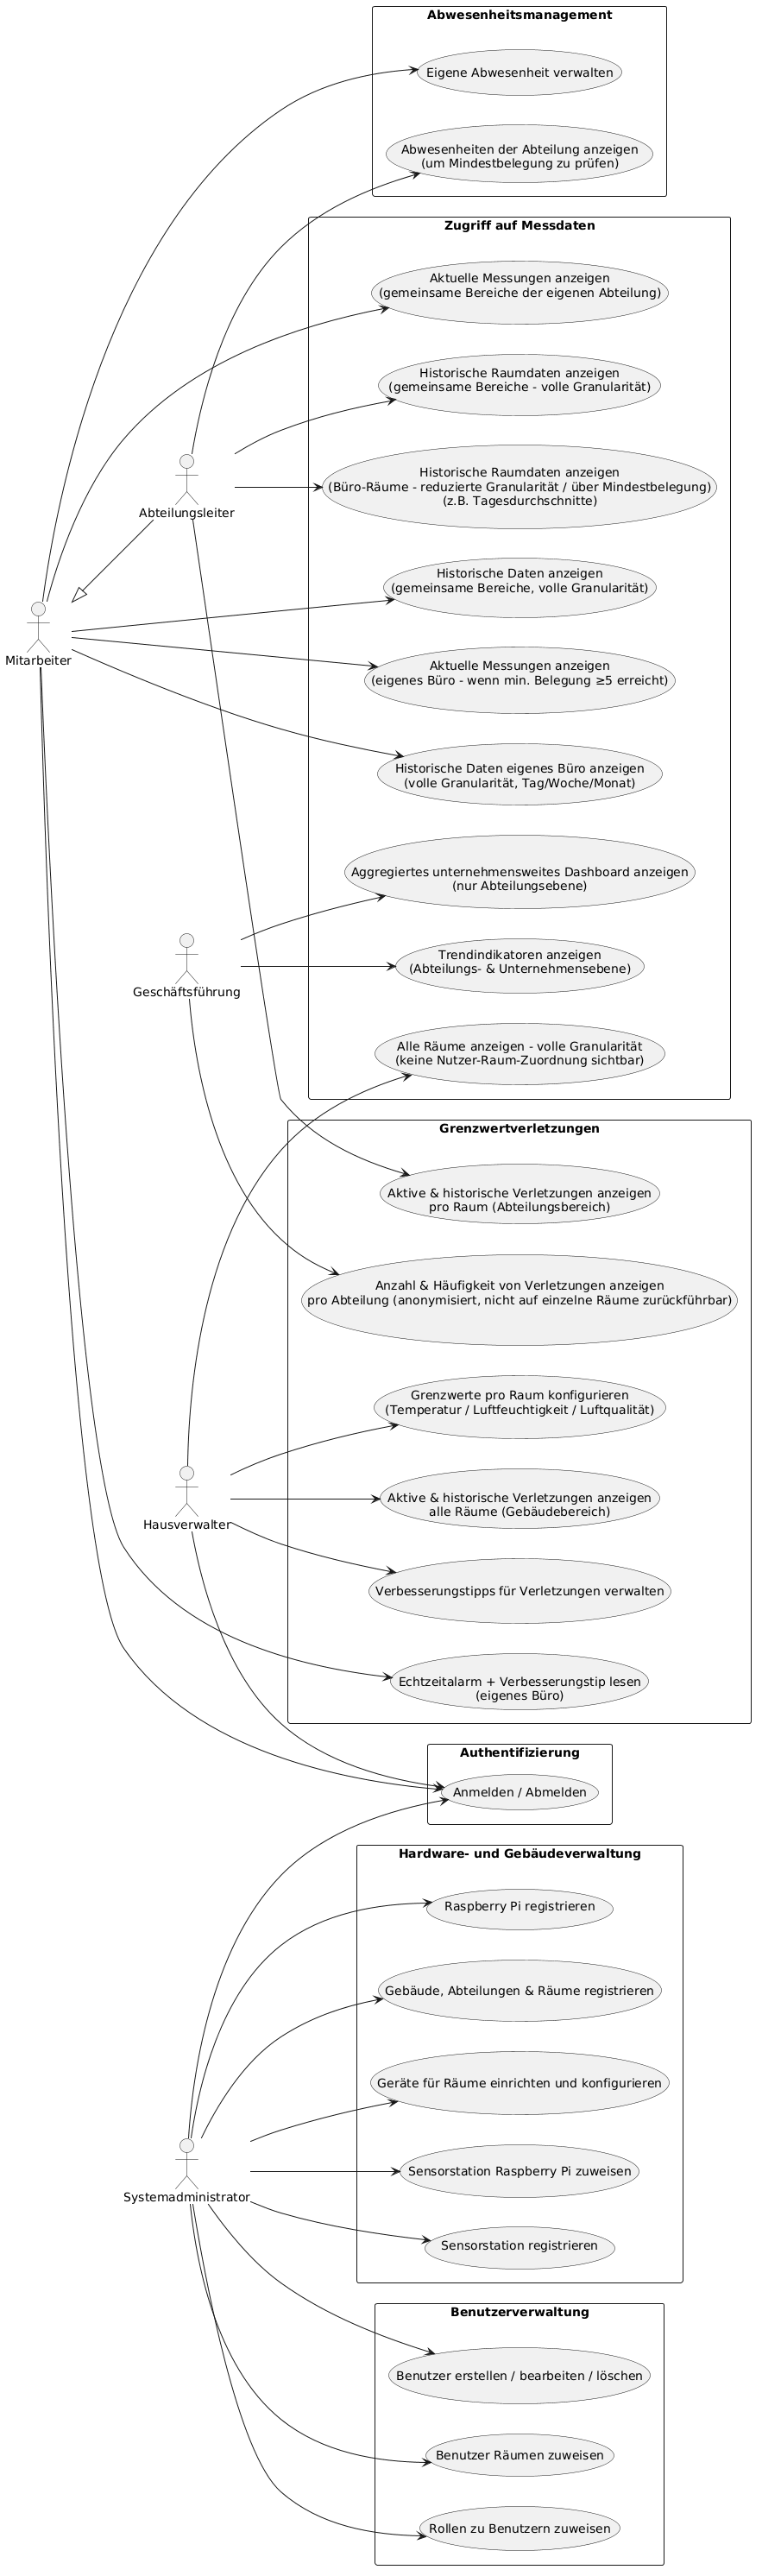
\includegraphics[width=0.3\textwidth]{images/Use Case Diagramm}
	\caption{Use Case Diagramm}
\end{figure}

\textit{Das vollständige Use Case Diagramm befindet sich als separates PNG im \texttt{/images} Ordner (Datei: \texttt{images/Use\_Case\_Diagramm.png}).}

\subsection{Akteure}
\begin{itemize}
	\item \textbf{Mitarbeiter:in} -- Basisrolle; hat Zugriff auf eigenes Büro (bei ausreichender Belegung) und Allgemeinflächen der eigenen Abteilung.
	\item \textbf{Abteilungsleitung} -- Erbt alle Rechte der Mitarbeiter:in; zusätzlich Abteilungsübersicht mit reduzierter Granularität für Büroräume.
	\item \textbf{Geschäftsführung} -- Nur firmenweite, aggregierte Sicht auf Abteilungsebene; keine Raumdetails, keine Userdaten.
	\item \textbf{Hausverwalter} -- Vollzugriff auf Raumklimadaten und Konfiguration; sieht ausdrücklich \emph{keine} Nutzer-Raum-Zuordnungen oder Abwesenheiten.
	\item \textbf{Systemadministrator} -- Vollzugriff auf Benutzer- und Geräteverwaltung; kein Zugriff auf Messdaten oder Grenzwertkonfiguration.
\end{itemize}

\subsection{Übersicht der Use Cases}

\begin{center}
	\begin{tabularx}{\textwidth}{lX}
		\toprule
		\textbf{Akteur} & \textbf{Use Cases} \\
		\midrule
		Mitarbeiter:in & Anmelden/Abmelden, aktuelle Messungen des eigenen Büros einsehen (nur bei Mindestbelegung $\geq$ 5), historische Daten des eigenen Büros einsehen, aktuelle und historische Messungen gemeinsamer Bereiche der eigenen Abteilung einsehen, Echtzeitalarme und Verbesserungstipps bei Grenzwertverletzungen lesen, eigene Abwesenheiten verwalten \\
		Abteilungsleitung & Historische Raumdaten von Büro-Räumen der Abteilung einsehen (reduzierte Granularität, z.\,B. Tagesdurchschnitte), historische Daten gemeinsamer Bereiche einsehen, aktive und historische Grenzwertverletzungen pro Raum im Abteilungsbereich einsehen, Abwesenheiten der Abteilung einsehen \\
		Geschäftsführung & Aggregiertes unternehmensweites Dashboard einsehen (auf Abteilungsebene), Trendindikatoren für Abteilungen und Unternehmen einsehen, anonymisierte Statistiken zu Grenzwertverletzungen pro Abteilung einsehen \\
		Hausverwalter & Alle Raumdaten mit voller Granularität einsehen (ohne Nutzer-Raum-Zuordnung), aktive und historische Grenzwertverletzungen aller Räume einsehen, Grenzwerte für Temperatur, Luftfeuchtigkeit und Luftqualität konfigurieren, Verbesserungstipps für Grenzwertverletzungen verwalten \\
		Systemadministrator & Gebäude, Abteilungen und Räume registrieren und verwalten, Raspberry Pis registrieren, Sensorstationen registrieren und Raspberry Pis zuweisen, Geräte für Räume konfigurieren, Benutzer erstellen/bearbeiten/löschen, Rollen zuweisen, Benutzer Räumen zuweisen \\
		\bottomrule
	\end{tabularx}
\end{center}

\section{Use Case Beschreibungen}
\subsection{UC-01: Raumklimadaten eigenes Büro einsehen}

\begin{itemize}
  \item \textbf{Akteur}: Mitarbeiter:in
  \item \textbf{Vorbedingung}: Nutzer:in ist eingeloggt und einem Büroraum zugeordnet. Mindestens 5 Personen des Raums sind aktuell anwesend (keine Abwesenheit erfasst).
  \item \textbf{Normalablauf}:
    \begin{enumerate}
      \item Nutzer:in öffnet die Raumansicht des eigenen Büros.
      \item System prüft die aktuelle Belegung des Raums.
      \item System zeigt aktuelle Messwerte (Temperatur, Luftfeuchtigkeit, Luftqualität) und Verlaufsdiagramme (Tages-/Wochen-/Monatsansicht) an.
      \item Konfigurierte Grenzwerte sind als Referenzlinien in den Diagrammen sichtbar.
      \item Aktive Grenzwertwarnungen werden prominent angezeigt, inkl. Raumklima-Tipps.
    \end{enumerate}
  \item \textbf{Alternativablauf -- Mindestbelegung nicht erfüllt}:
    \begin{enumerate}
      \item System erkennt, dass die Belegung unter 5 Personen liegt.
      \item System zeigt Hinweis: ``Keine Daten verfügbar -- Datenschutzbedingungen nicht erfüllt.''
      \item Keine Messdaten werden angezeigt.
    \end{enumerate}
  \item \textbf{Alternativablauf -- Verbindungsausfall}:
    \begin{enumerate}
      \item Für einen bestimmten Zeitraum fehlen Messdaten (z.B. Raspberry Pi offline).
      \item System markiert Lücken in den Verlaufsdiagrammen deutlich (z.B. grau hinterlegte Bereiche).
    \end{enumerate}
\end{itemize}

\vspace{0.5em}
\subsection{UC-02: Raumklimadaten Allgemeinflächen einsehen}

\begin{itemize}
  \item \textbf{Akteur}: Mitarbeiter:in, Abteilungsleitung
  \item \textbf{Vorbedingung}: Nutzer:in ist eingeloggt und einer Abteilung zugeordnet.
  \item \textbf{Normalablauf}:
    \begin{enumerate}
      \item Nutzer:in wählt eine Allgemeinfläche (Konferenzraum, Aufenthaltsraum etc.) der eigenen Abteilung aus.
      \item System zeigt aktuelle Messwerte und Verlaufsdiagramme in voller Granularität an.
      \item Keine Datenschutzeinschränkungen -- Daten sind immer verfügbar.
    \end{enumerate}
\end{itemize}

\vspace{0.5em}
\subsection{UC-03: Abteilungsübersicht einsehen}

\begin{itemize}
  \item \textbf{Akteur}: Abteilungsleitung
  \item \textbf{Vorbedingung}: Nutzer:in ist als Abteilungsleitung eingeloggt.
  \item \textbf{Normalablauf}:
    \begin{enumerate}
      \item Abteilungsleitung öffnet die Abteilungsübersicht.
      \item System zeigt eine vergleichende Darstellung aller Räume der Abteilung (aktuelle Messwerte, Anzahl aktiver Warnungen).
      \item Für Büros oberhalb der Mindestbelegung: Verlaufsansichten in reduzierter Granularität (Tagesdurchschnitte).
      \item Für Allgemeinflächen: Verlaufsansichten in voller Granularität.
      \item Aktive und vergangene Grenzwertverletzungen auf Raumebene sind einsehbar.
    \end{enumerate}
\end{itemize}

\vspace{0.5em}
\subsection{UC-04: Grenzwertwarnung -- Auslösung und Anzeige}

\begin{itemize}
  \item \textbf{Akteur}: Raspberry Pi (technisch), Mitarbeiter:in / Abteilungsleitung (sichtbar)
  \item \textbf{Vorbedingung}: Grenzwerte sind für den betroffenen Raum konfiguriert. Sensorstation ist aktiv und verbunden.
  \item \textbf{Normalablauf}:
    \begin{enumerate}
      \item Raspberry Pi empfängt Messdaten von der Sensorstation.
      \item Raspberry Pi prüft Messwerte gegen konfigurierte Grenzwerte mit Noise-Filter (kein Auslösen bei kurzfristigen Ausreißern).
      \item Bei bestätigter Grenzwertüberschreitung: Raspberry Pi setzt Warnstatus und sendet diesen an die Sensorstation und die Webapp.
      \item Sensorstation: LED wechselt auf Rot, Display zeigt Warnmodus mit Hinweis und Tipp.
      \item Webapp: Warnung wird prominent für alle Nutzer:innen des betroffenen Raums angezeigt, inkl. konfiguriertem Raumklima-Tipp.
      \item Abteilungsleitung sieht Warnung in der Abteilungsübersicht.
    \end{enumerate}
  \item \textbf{Alternativablauf -- Warnung aufheben}:
    \begin{enumerate}
      \item Messwerte kehren dauerhaft in den Normalbereich zurück.
      \item Raspberry Pi hebt Warnstatus auf und informiert Sensorstation und Webapp.
      \item LED wechselt auf Grün, Warnmeldung in der Webapp verschwindet. Vergangene Verletzung bleibt historisch gespeichert.
    \end{enumerate}
  \item \textbf{Designentscheidung}: Eine Grenzwertwarnung wird erst ausgelöst, wenn ein Grenzwert über einen konfigurierbaren Zeitraum (z.B. 3 aufeinanderfolgende Messungen) überschritten wird. Dadurch werden kurzfristige Ereignisse (Fenster kurz öffnen, Atemstoß auf Sensor) gefiltert.
\end{itemize}

\vspace{0.5em}
\subsection{UC-05: Grenzwerte konfigurieren}

\begin{itemize}
  \item \textbf{Akteur}: Gebäudeadministration
  \item \textbf{Vorbedingung}: Nutzer:in ist als Gebäudeadmin eingeloggt. Raum und Sensorstation sind im System angelegt.
  \item \textbf{Normalablauf}:
    \begin{enumerate}
      \item Gebäudeadmin öffnet die Konfigurationsansicht eines Raums.
      \item Admin setzt oder ändert obere Grenzwerte für Temperatur, Luftfeuchtigkeit und Luftqualität. Untere Grenzwerte sind optional.
      \item System speichert die neuen Grenzwerte in der PostgreSQL-Datenbank.
      \item System informiert den zuständigen Raspberry Pi über die Änderung per REST-Benachrichtigung.
      \item Raspberry Pi ruft die aktualisierten Grenzwerte ab und speichert sie lokal in der SQLite-Datenbank.
    \end{enumerate}
\end{itemize}

\vspace{0.5em}
\subsection{UC-06: Abwesenheit eintragen}

\begin{itemize}
  \item \textbf{Akteur}: Mitarbeiter:in
  \item \textbf{Vorbedingung}: Nutzer:in ist eingeloggt und einem Büroraum zugeordnet.
  \item \textbf{Normalablauf}:
    \begin{enumerate}
      \item Mitarbeiter:in trägt eine Abwesenheit (Urlaub, Krankheit, etc.) stunden- oder tageweise ein.
      \item System prüft, ob durch diese Abwesenheit die Mindestbelegung (5 Personen) im Büroraum unterschritten wird.
      \item Wenn ja: System informiert den zuständigen Raspberry Pi. Ab diesem Zeitpunkt werden keine Messdaten für diesen Raum persistent gespeichert oder übertragen.
      \item Wenn nein: Keine Änderung am Datenspeicherverhalten.
    \end{enumerate}
\end{itemize}

\vspace{0.5em}
\subsection{UC-07: Geräte anlegen und konfigurieren}

\begin{itemize}
  \item \textbf{Akteur}: Systemadministration
  \item \textbf{Vorbedingung}: Nutzer:in ist als Systemadmin eingeloggt. Gebäudestruktur (Gebäude, Abteilungen, Räume) ist bereits angelegt.
  \item \textbf{Normalablauf}:
    \begin{enumerate}
      \item Systemadmin legt ein neues Raspberry Pi-Objekt an. System generiert automatisch eine eindeutige ID.
      \item Systemadmin ordnet den Raspberry Pi einem Raum zu.
      \item Systemadmin legt eine neue Sensorstation an. System generiert automatisch eine eindeutige ID.
      \item Systemadmin ordnet die Sensorstation dem Raspberry Pi zu.
      \item Die generierten IDs werden für die physische Konfiguration der Geräte verwendet (hardcoded auf Arduino, conf.yaml auf Raspberry Pi).
    \end{enumerate}
\end{itemize}
\newpage
\section{Klassendiagramm V1}

\begin{figure}[h!]
	\centering
	
\includegraphics[width=0.8\textwidth]{images/climate-canary-webapp-backend.png}
	\caption{Klassendiagramm V1}
	\label{fig:climate-canary-webapp-backend}
\end{figure}

\textit{Das vollständige Klassendiagramm befindet sich als separates Draw.io im GitLab Wiki (Datei: \texttt{climate-canary-webapp-backend.drawio}).}

\subsection{Klassenbeschreibungen}

\begin{itemize}
  \item \textbf{ViolationStatus} -- Enum: ACTIVE, RESOLVED.
  \item \textbf{Role} -- Enum: EMPLOYEE, DEPARTMENT\_LEAD, MANAGEMENT, BUILDING\_ADMIN, SYSTEM\_ADMIN.
  \item \textbf{AbsenceType} -- Enum: HOLIDAY, SICKNESS, PARENTAL\_LEAVE, OTHER.
  \item \textbf{AbsenceStatus} -- Enum: PLANNED, APPROVED, REJECTED, CANCELLED.
  \item \textbf{RoomType} -- Enum: OFFICE, COMMON\_AREA, OTHER.
  \item \textbf{DeviceStatus} -- Enum: ONLINE, OFFLINE, MAINTENANCE.
  \item \textbf{Metric} -- Enum: TEMPERATURE, HUMIDITY, AIR\_QUALITY.

  
  \item \textbf{User} -- Repräsentiert einen Systembenutzer.\\Attribute: id, firstName, lastName, email, passwordHash, role, departmentIds, roomId.\\Assoziationen: gehört einer oder mehreren Abteilungen an, ist einem Büroraum zugeordnet, hat Abwesenheiten.
  \\\small{Designentscheidung: Ein User kann mehreren Abteilungen angehören, um beispielsweise Management- oder Gebäudeadministrationsrollen zu ermöglichen, die Zugriff auf mehrere Abteilungen benötigen.}
  \item \textbf{Absence} -- Repräsentiert eine Abwesenheit eines Users.\\Attribute: id, userId, startDate, endDate, absenceType, absenceStatus.\\Assoziationen: referenziert einen User.
  \item \textbf{Building} -- Repräsentiert ein Gebäude.\\Attribute: id, name, addressId.\\Assoziationen: hat eine Addresse, wird von mehreren Abteilungen und Räumen referenziert.
  \item \textbf{Address} -- Repräsentiert eine Adresse.\\Attribute: id, country, zipCode, city, street, houseNumber, extra.\\Assoziationen: wird von einem Gebäude referenziert.
  \item \textbf{Department} -- Repräsentiert eine Abteilung.\\Attribute: id, name, buildingId.\\Assoziationen: gehört zu einem Gebäude, wird von mehreren Räumen und Usern referenziert.
  \item \textbf{Room} -- Repräsentiert einen Raum.\\Attribute: id, name, roomType, departmentId, minOccupancy (default: 5 für Büroräume), raspberryPiId.\\Assoziationen: hat einen Raspberry Pi, wird von Grenzwerten, Grenzwertüberschreitungen und einem RaspberryPi referenziert.
  \item \textbf{RaspberryPi} -- Repräsentiert einen Raspberry Pi.\\Attribute: id (generiert), roomId, ipAddress, deviceStatus, sensorStationIds.\\Assoziationen: hat Sensorstationenen, Grenzwerte werden über die Raumzuweisung verwaltet.
  \item \textbf{SensorStation} -- Repräsentiert eine Sensorstation (Arduino).\\Attribute: id (generiert, hardcoded auf Arduino), raspberryPiId, deviceStatus.\\Assoziationen: gehört zu einem Raspberry Pi, wird von Messunge und einem RaspberryPi referenziert.
  \item \textbf{Measurement} -- Repräsentiert einen Messdatenpunkt.\\Attribute: id, sensorStationId, timestamp, temperature, humidity, airQuality.\\Assoziationen: referenziert eine Sensorstation, wird von ThresholdViolation referenziert. (Wird nur bei erfüllter Datenschutzbedingung persistent gespeichert.)
  \item \textbf{Threshold} -- Repräsentiert Grenzwerte für einen Raum.\\Attribute: id, roomId, metric, upperBound, lowerBound (optional).\\Assoziationen: referenziert einen Raum, wird von ThresholdViolation referenziert, hat mehrere ClimateHints.
  \item \textbf{ThresholdViolation} -- Repräsentiert eine aktive oder historische Grenzwertverletzung.\\Attribute: id, roomId, thresholdId, startTime, endTime (null wenn noch aktiv), metric, value, violationStatus, measurementIds.\\Assoziationen: referenziert einen Raum und einen Threshold und mehrere Messungen.\\\small{Designentscheidung: mehrere Measurements müssen herangezogen werden, um kurze Extremwerte zu filtern. Eine Verletzung wird erst bestätigt, wenn z.B. 3 aufeinanderfolgende Messungen den Grenzwert überschreiten.}
  \item \textbf{ClimateHint} -- Repräsentiert einen Raumklima-Tipp.\\Attribute: id, metric, hintText.\\Assoziationen: wird von einem oder mehreren Threshholds referenziert. (Wird bei Grenzwertverletzungen angezeigt.)

\end{itemize}

\subsection{Wichtige Assoziationen}
\begin{itemize}
  \item \texttt{Building} $1$ -- $*$ \texttt{Department}: Ein Gebäude hat mehrere Abteilungen.
  \item \texttt{Department} $1$ -- $*$ \texttt{Room}: Eine Abteilung hat mehrere Räume.
  \item \texttt{Department} $1$ -- $*$ \texttt{User}: Eine Abteilung hat mehrere User.
  \item \texttt{Room} $1$ -- $0..1$ \texttt{RaspberryPi}: Ein Raum hat maximal einen Raspberry Pi.
  \item \texttt{RaspberryPi} $1$ -- $*$ \texttt{SensorStation}: Ein Raspberry Pi kann mehrere Sensorstationen verwalten (im Prototyp: eine).
  \item \texttt{SensorStation} $1$ -- $*$ \texttt{Measurement}: Eine Sensorstation produziert viele Messdaten.
  \item \texttt{Room} $1$ -- $*$ \texttt{Threshold}: Ein Raum hat Grenzwerte pro Messgröße.
  \item \texttt{User} $1$ -- $*$ \texttt{Absence}: Ein User kann mehrere Abwesenheiten haben.
\end{itemize}

\subsection{Löschen von Daten}
\begin{itemize}
  \item Wird ein User gelöscht, werden seine Abwesenheiten ebenfalls gelöscht (CASCADE).
  \item Wird eine Sensorstation gelöscht, werden ihre Messdaten ebenfalls gelöscht (CASCADE). Historische Grenzwertverletzungen bleiben erhalten (roomId Referenz bleibt bestehen).
  \item Wird ein Raum gelöscht, werden alle zugehörigen Messdaten, Grenzwerte und Grenzwertverletzungen gelöscht (CASCADE).
  \item Wird ein Raspberry Pi aus einem Raum entfernt, bleiben historische Messdaten erhalten; der Raspberry Pi-Eintrag bleibt im System, bis er explizit gelöscht wird.
  \item Messdaten, die aufgrund der Datenschutzbedingung (Mindestbelegung) nicht gespeichert wurden, existieren nie persistent -- sie müssen also nicht gelöscht werden.
\end{itemize}

\section{GUI Prototyp}

\textit{Der vollständige GUI Prototyp (Mockups) befindet sich als separates Dokument im GitLab Wiki. Hier folgt eine textuelle Beschreibung der Kernansichten.}

\subsection{Login}
\begin{itemize}
  \item Einfache Login-Maske mit E-Mail und Passwort.
  \item Nach Login: Weiterleitung auf rollenabhängiges Dashboard.
\end{itemize}

\subsection{Dashboard (Mitarbeiter:in)}
\begin{itemize}
  \item Übersichtskacheln: Eigenes Büro (aktuelle Temperatur, Luftfeuchtigkeit, Luftqualität) + Allgemeinflächen der Abteilung.
  \item Prominente Warnanzeige wenn aktive Grenzwertverletzung im eigenen Büro vorhanden.
  \item Hinweisbox wenn Bürodaten wegen Datenschutz nicht verfügbar sind.
  \item Navigation zu: Verlaufsansicht, Abwesenheitsverwaltung.
\end{itemize}

\begin{itemize}
  \item Liniendiagramm für Temperatur, Luftfeuchtigkeit, Luftqualität über wählbaren Zeitraum (Tag / Woche / Monat).
  \item Grenzwerte als horizontale Referenzlinien eingeblendet.
  \item Vergangene Grenzwertverletzungen farblich markiert.
  \item Datenlücken (Datenschutz, Ausfall) klar als graue Bereiche gekennzeichnet.
  \item Granularität abhängig von Rolle (Mitarbeiter: Rohdaten; Abteilungsleitung: Tagesdurchschnitte für Büros).
\end{itemize}

\subsection{Dashboard (Abteilungsleitung)}
\begin{itemize}
  \item Rasteransicht aller Räume der Abteilung mit aktuellen Messwerten und Warnstatus.
  \item Anzahl aktiver Grenzwertverletzungen pro Raum.
  \item Verlinkung zu Raumdetailansicht mit reduzierter Granularität für Büros.
\end{itemize}

\subsection{Dashboard (Höheres Management)}
\begin{itemize}
  \item Firmenweites Dashboard: Aggregierte Werte nach Abteilungen.
  \item Balkendiagramm: Anzahl Grenzwertverletzungen pro Abteilung (anonymisiert).
  \item Trendlinie über Wochen/Monate.
\end{itemize}

\subsection{Konfigurationsansicht (Gebäudeadmin)}
\begin{itemize}
  \item Liste aller Räume mit aktuellen Grenzwerten.
  \item Inline-Bearbeitung der Grenzwerte pro Raum und Messgröße.
  \item Tipp-Verwaltung: Liste, Erstellen, Bearbeiten, Löschen von Raumklima-Tipps.
\end{itemize}

\subsection{Gerätemanagement (Systemadmin)}
\begin{itemize}
  \item Übersicht aller Raspberry Pis und Sensorstationen mit Status (Online/Offline).
  \item Anlegen neuer Geräte inkl. automatisch generierter ID.
  \item Zuweisung von Sensorstationen zu Raspberry Pis und Räumen.
  \item Benutzerverwaltung: Nutzer:innen anlegen, Rollen zuweisen, Räumen zuordnen.
\end{itemize}

\section{Projektplan}

\subsection{Verantwortlichkeiten}

\begin{center}
\begin{tabularx}{\textwidth}{lX}
  \toprule
  \textbf{Person} & \textbf{Zuständigkeit} \\
  \midrule
  Maria Kuhn      & Arduino-Entwicklung (C/C++, BLE-Protokoll), Frontend (React/TS) \\
  Fabienne Schedler & Frontend (React/TS, PrimeReact, GUI-Prototyp, Mobile-First) \\
  Emma Danko      & Raspberry Pi (Python, BLE Central, SQLite), Backend (Spring Boot) \\
  Prahbdip Singh  & Raspberry Pi (Python, REST-Schnittstellen, Docker), Backend (Spring Boot, PostgreSQL) \\
  Adriano Paganini & Arduino-Entwicklung (C/C++, Display/LED/Buttons), Backend (Spring Boot, API Design) \\
  \midrule
  \textbf{Alle} & Softwarekonzept, Testing, Dokumentation, Code Review \\
  \bottomrule
\end{tabularx}
\end{center}

\subsection{Meilensteine und Zeitplan}

\begin{center}
\begin{tabularx}{\textwidth}{llX}
  \toprule
  \textbf{Datum} & \textbf{Meilenstein} & \textbf{Inhalt} \\
  \midrule
  12.03.2026 & \textbf{Konzept V1} & Systemüberblick, Use Cases, Klassendiagramm V1, GUI Prototyp, Projektplan \\
  19.03.2026 & \textbf{Konzept V2} & Sequenzdiagramme, API Dokumentation, Ausfallssicherheit, Klassendiagramm V2 \\
  27.03.2026 & \textbf{Konzept Final} & Überarbeitetes Gesamtkonzept nach Feedback \\
  \midrule
  KW 14--15  & \textbf{M1: Hardware Setup} & Arduino + Sensoren funktionsfähig; BLE-Übertragung zum RPi; Raspberry Pi OS + Docker eingerichtet \\
  KW 16--17  & \textbf{M2: Backend Grundgerüst} & Spring Boot Skeleton aufgesetzt; PostgreSQL Datenbankschema implementiert; Basis-REST-API (OpenAPI); Login/Rollen \\
  KW 18--19  & \textbf{M3: Datenfluss End-to-End} & Kompletter Datenfluss Arduino $\to$ RPi $\to$ Backend funktionsfähig; Grenzwertberechnung am RPi; Datenschutzlogik \\
  KW 20--21  & \textbf{M4: Frontend + Warnungen} & Rollenabhängige Dashboards; Verlaufsdiagramme; Grenzwertwarnungen in Webapp und auf Sensorstation \\
  KW 22--23  & \textbf{M5: Ausfallssicherheit + Testing} & Ausfallszenarien abgesichert; SonarQube integriert; $\geq$ 65\% Testabdeckung \\
  KW 24      & \textbf{M6: Finalisierung} & Bugfixes; Dokumentation vollständig; finale Abgabe (18.06.2026) \\
  \bottomrule
\end{tabularx}
\end{center}

\subsection{Inkrementelle Entwicklung}
\begin{itemize}
  \item Wir entwickeln das System in zwei parallelen Tracks: \textbf{Hardware-Track} (Arduino + Raspberry Pi) und \textbf{Software-Track} (Backend + Frontend).
  \item Beide Tracks werden ab M3 integriert.
  \item Jede Woche wird im Team eine kurze Sync-Session abgehalten, um Fortschritte und Blocker zu besprechen.
  \item GitLab wird für Issues, Merge Requests und Code Review genutzt. Das Wiki enthält alle Konzept-Dokumente.
  \item SonarQube wird ab Beginn der Backend-Entwicklung (KW 14) integriert, nicht erst kurz vor der Abgabe.
\end{itemize}

\subsection{Zusätzliche Aufgaben}
\begin{itemize}
  \item Zwischenbericht: Einplanen in KW 18 (nach M3).
  \item Abschlussbericht: Einplanen in KW 23--24.
  \item Präsentation: Vorbereitung in KW 24.
  \item Testdaten: Realistische Testdaten für alle Rollen und Szenarien werden in KW 20 erstellt.
\end{itemize}

\end{document}
